% Generated by TeXFlow — do not edit.
% Changes will be overwritten on next compile.
% Use the TeXFlow edit() and layout() tools to modify the document.
\documentclass[10pt, conference, letterpaper]{IEEEtran}

\IEEEoverridecommandlockouts
\markboth{Anonymous}{Patient-Independent TinyML ECG Classification: Generalization, Robustness, Quantization, and ESP32-S3 Deployment Trade-offs}
\title{Patient-Independent TinyML ECG Classification:\\
Generalization, Robustness, Quantization, and ESP32-S3 Deployment Trade-offs}
\author{
\IEEEauthorblockN{1st Given Name Surname}
\IEEEauthorblockA{\textit{Dept. name of organization}\\
\textit{Name of organization}\\
City, Country \\
email address or ORCID}
\and
\IEEEauthorblockN{2nd Given Name Surname}
\IEEEauthorblockA{\textit{Dept. name of organization}\\
\textit{Name of organization}\\
City, Country \\
email address or ORCID}
\and
\IEEEauthorblockN{3rd Given Name Surname}
\IEEEauthorblockA{\textit{Dept. name of organization}\\
\textit{Name of organization}\\
City, Country \\
email address or ORCID}
\and
\IEEEauthorblockN{4th Given Name Surname}
\IEEEauthorblockA{\textit{Dept. name of organization}\\
\textit{Name of organization}\\
City, Country \\
email address or ORCID}
}

\usepackage{amsmath}
\usepackage{amssymb}
\usepackage{booktabs}
\usepackage{placeins}
\usepackage{graphicx}
\usepackage{url}
\usepackage[colorlinks=true,linkcolor=black,urlcolor=blue,citecolor=blue]{hyperref}

\begin{document}
\maketitle

\begin{abstract}
Low-cost wearable ECG screening aims at early detection of abnormal rhythms on sub-\$15 microcontrollers, but must balance accuracy, size and latency. We evaluate four architectures (1D-CNN, LSTM, GRU, TCN) for 3-class beat classification (Normal/APB/PVC) on MIT-BIH using \emph{identical} patient-level folds. Five experiments cover patient-independent grouped CV ($5\times2$), noise robustness (SNR 0--40\,dB, 5 artifacts $\times$ 3 front-ends), external validation on SVDB (N/V-macro), paired FP32$\rightarrow$INT8 quantization, and on-device measurement on ESP32-S3. APB remains the minority bottleneck (grouped-CV APB F1 $0.14$--$0.28$; mitigation lifts CNN APB to $0.73$ on a single split). INT8 degrades macro by $0.21$--$0.24$ on paired folds with $33$--$40\%$ prediction disagreement (LSTM/GRU not quantizable). On ESP-NN-optimized kernels the same silicon classifies a 1-s window in $184$\,ms (CNN) / $293$\,ms (TCN)---inside the $500$-ms hop that 50\% window overlap imposes on streaming (hop-based RTF $0.38$/$0.60$)---once the learned denoiser is replaced by a ${\sim}5$\,ms Butterworth; with the denoiser in-loop the pipeline sits at RTF $1.00$/$1.22$, and float32 LSTM/GRU fail under either framing ($\geq1.55$). Kernel optimization, not architecture, was the deployment bottleneck. Butterworth front-end ($0$\,KB, ${\sim}5$\,ms) dominates the learned denoiser ($19$\,KB, $315$\,ms on ESP-NN).
\end{abstract}

\section{Introduction}

Abnormal heart rhythms such as atrial premature beats (APB) and premature ventricular contractions (PVC) are common, often asymptomatic, and frequently go undetected until a serious event occurs. Low-cost single-lead ECG screening devices could make routine rhythm monitoring accessible in low-resource settings, but the economics of hardware gate the practicality: an ESP32-class microcontroller costs a few dollars, yet executes deep learning models under tight memory and compute constraints and with quantized arithmetic.

Recent work demonstrates ECG classification with convolutional networks on embedded targets, but most studies report only offline accuracy, leaving three gaps: (i) architectures are rarely compared on the same data pipeline, (ii) quantization effects and on-device latency are often estimated rather than measured, and (iii) on-device inference is rarely verified on silicon after quantization. This paper addresses all three: four architectures (1D-CNN, LSTM, GRU, TCN) trained on identical patient-level MIT-BIH splits and evaluated across five experiments---grouped cross-validation, noise robustness, external SVDB generalization, paired FP32-to-int8 quantization, and measured on-device execution on an ESP32-S3 (\S IV details the protocol).


\section{Related Work}

Beat-level ECG classification on MIT-BIH is a mature problem; convolutional and recurrent models report high per-class F1 for Normal and PVC classes, with atrial beats typically the most difficult minority class \cite{mitdb,annaram}. For deployment, TensorFlow Lite Micro enables int8 inference on microcontrollers \cite{davidson2021tflm}, and prior ESP32 ECG studies demonstrate the feasibility of a single CNN on this class of hardware \cite{esp32ecg}. Rhythm-level atrial fibrillation detection is conventionally addressed on longer windows with dedicated AF databases \cite{moody1983new}; beat-level and rhythm-level tasks are deliberately kept separate in this work, and rhythm-level AF detection is not evaluated here. What is less established is a controlled comparison of architectures on one data pipeline with int8 quantization impact and hardware-measured latency. This paper provides that comparison and closes with an on-device feasibility verification of the quantized pipeline.

Convolutional and recurrent approaches to heartbeat classification now report strong results on MIT-BIH, from patient-specific 1-D CNNs \cite{kiranyaz2016} to cardiologist-level recurrent and convolutional models trained on large ambulatory corpora \cite{hannun2019,rajpurkara2017} and on 12-lead ECG \cite{ribeiro2020}; surveys of the area \cite{luz2016,acharya2017,yildirim2018} and of the monitoring-system design space \cite{serhani2020} consistently note that the atrial (minority) class remains the main difficulty. Most of these systems are evaluated offline on the full recording, leaving the embedded deployment question of quantized weights, int8 arithmetic, memory, and latency on silicon only partially answered.

For edge deployment the relevant tooling is now mature: integer-arithmetic-only quantization \cite{jacob2018,krishnamoorthi2018} makes int8 inference practical on microcontroller-class parts, TensorFlow Lite Micro provides the runtime \cite{davidson2021tflm}, TinyML design guidance targets the flash and memory budgets we report \cite{warden2020}, and calibrated probabilities matter for thresholded decisions \cite{guo2017,naeini2015}. The ESP32-S3's reference documentation defines the ADC, DMA, and low-power modes the firmware relies on \cite{espressifs3}.

\begin{table}[t]
\centering
\resizebox{\linewidth}{!}{
\begin{tabular}{l c c c c c c c}
\toprule
Work & Pat.-ind & Ext. & Noise & Quant & MCU & Calib & Latency \\
\midrule
Kiranyaz 2016 & --- & --- & --- & --- & --- & --- & --- \\
Hannun 2019 & --- & $\checkmark$ & --- & --- & --- & --- & --- \\
Davidson 2021 (TFLM) & --- & --- & --- & $\checkmark$ & $\checkmark$ & --- & $\checkmark$ \\
ESP32 ECG '19 & --- & --- & $\checkmark$ & $\checkmark$ & $\checkmark$ & --- & est \\
\textbf{This work} & \textbf{$\checkmark$} & \textbf{$\checkmark$} & \textbf{$\checkmark$} & \textbf{$\checkmark$} & \textbf{$\checkmark$} & \textbf{$\checkmark$} & \textbf{$\checkmark$} \\
\bottomrule
\end{tabular}
}
\caption{Prior-work gap: patient-independent CV, external, noise (5 artifacts $\times$ 3 front-ends), paired quant, real S3, calibration (ECE/NLL/Brier), measured latency.}
\label{tab:gap}
\end{table}


\section{Methods}

\subsection{Data and labels}

Beat-level training uses the MIT-BIH Arrhythmia Database \cite{mitdb,moody1990} (48 recordings, 360 Hz, MLII lead), part of the public PhysioNet archive \cite{goldberger2000}. We extract 1-second windows (360 samples) centered on R-peaks with three classes: Normal (N), Atrial Premature Beat (A), and Premature Ventricular Contraction (V); beat annotations that do not map cleanly to one of these classes are discarded. Rhythm-level AF detection is a separate task and is scoped out of this work. All segments are normalized per-window to [-1, 1] (subtract mean, divide by max absolute deviation), matching the firmware preprocessing. Figure~\ref{fig:methodology} outlines the complete methodology from data preparation through patient-level evaluation to on-device verification.

\begin{figure}[t]
\centering
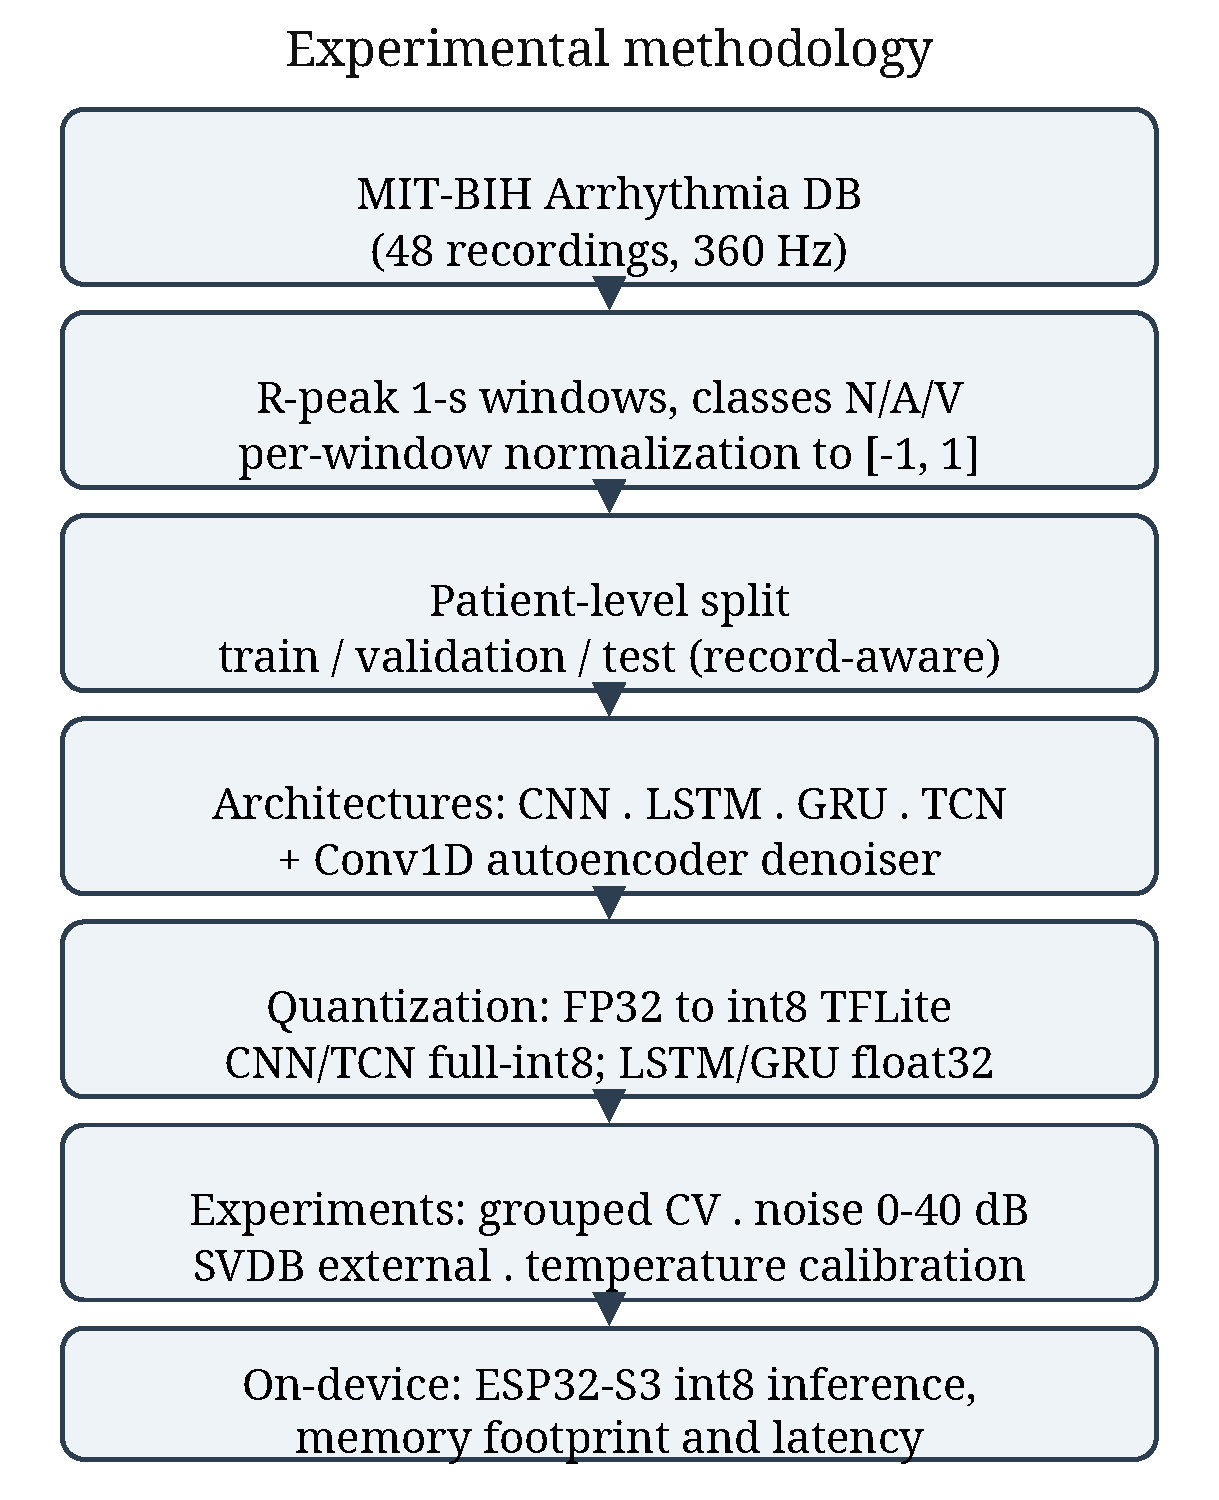
\includegraphics[width=0.92\columnwidth]{figures/fig_methodology.pdf}
\caption{Overview of the experimental methodology, from MIT-BIH preprocessing through patient-level evaluation, quantization, and on-device verification.}
\label{fig:methodology}
\end{figure}
\begin{equation}
\hat{x}_i = \frac{x_i - \mu}{\max_j |x_j - \mu|}, \quad \mu = \frac{1}{L}\sum_{i=1}^{L} x_i
\end{equation}


\subsection{Signal quality gate}

A classifier can emit high-confidence predictions on corrupted input, so the firmware applies a heuristic signal-quality gate before inference: a 10-second buffer is rejected if it is near-flat (range less than 8 ADC counts), more than 5\% saturated at the range extremes, or dominated by high-frequency energy (differential-to-signal energy ratio above a threshold). Rejected buffers never reach the network.

\begin{equation}
\text{range} = \max_i x_i - \min_i x_i, \qquad \text{ratio} = \frac{\sum_{i=1}^{L-1} (x_{i+1}-x_i)^2}{\sum_{i=1}^{L} (x_i - \bar{x})^2}
\end{equation}

The ratio is an inexpensive proxy for high-frequency corruption such as muscle artifact or baseline wander \cite{clifford2006}.


\subsection{Models}\label{sec:methods-models}

Four architectures share one head (global pooling, dense 64, dropout 0.5, softmax) and one training schedule (Adam \cite{kingma2015}, 1e-3, batch 64, early stopping): CNN (three Conv1D blocks, 32/64/128 filters with batch normalization \cite{ioffe2015}, kernel 5), LSTM \cite{hochreiter1997} and GRU (one Conv1D block followed by 64 recurrent units), and TCN (a temporal convolutional network with two dilated causal blocks and residual connections \cite{bai2018}). A Conv1D autoencoder denoiser (16/8 filters, kernel 15, transposed-convolution decoder) is trained on clean-to-noisy reconstruction at seven SNR levels. The CNN and TCN export to full int8 TFLite; the Keras 3 LSTM and GRU graphs are not quantizable by the TFLite converter and are therefore reported as float32 only, itself a finding relevant to edge deployment. For on-device timing we additionally re-exported both RNNs through fused sequence layers (UNIDIRECTIONAL\_SEQUENCE\_LSTM/GRU builtins) via a static-shape concrete-function conversion with weights transferred unchanged; these FP32 variants are what Table~\ref{tab:deploy} benchmarks. Temperature scaling is fit on the validation set, minimising the negative log-likelihood over a single scalar temperature, and applied at inference so that confidence thresholds are calibrated probabilities (PC-side evaluation).

\begin{equation}
\sigma_n = \sigma_s \cdot 10^{-\mathrm{SNR}/20}, \qquad \tilde{x} = x + n, \quad n \sim \mathcal{N}(0, \sigma_n^2)
\end{equation}

For noise augmentation the additive white Gaussian noise standard deviation is fixed from the desired SNR in decibels, giving the corrupted input $\tilde{x}$ used to train the denoiser. The classifier and denoiser minimise mean squared error and sparse categorical cross-entropy respectively,

\begin{equation}
\mathcal{L}_{\mathrm{den}} = \frac{1}{N}\sum_{i=1}^{N} \| x_i - g(\tilde{x}_i) \|_2^2, \qquad \mathcal{L}_{\mathrm{cls}} = -\frac{1}{N}\sum_{i=1}^{N}\log p_{\hat{y}_i}(x_i)
\end{equation}

\begin{equation}
q = \mathrm{clip}\big(\mathrm{round}(r/s) + z,\ q_{\min}, q_{\max}\big), \qquad r \approx s\,(q - z)
\end{equation}

The affine int8 map (5) is applied identically in the TFLite converter and the firmware's manual input conversion, so on-device tensors match the offline converter exactly.

\begin{equation}
\begin{split}
p_k &= \frac{\exp\big(z_k / T\big)}{\sum_j \exp\big(z_j / T\big)},\\
\mathrm{ECE} &= \sum_{m=1}^{M} \frac{|B_m|}{N}\,\big|\mathrm{acc}_m - \mathrm{conf}_m\big|.
\end{split}
\end{equation}


\subsection{Hardware and deployment}

The target device is an ESP32-S3 (N16R8: 16 MB flash, 8 MB PSRAM). ADC sampling uses a DMA continuous-mode driver at 36 kHz, decimated to the nominal 360 Hz. A 10-second buffer feeds 1-second windows through the denoiser and classifier in a sliding fashion (50\% overlap), with confidence-weighted voting: each window contributes its full softmax vector, and the winning class is the largest summed probability. Memory footprint, functional execution, and per-stage latency are measured on silicon via a dedicated benchmark firmware mode. The firmware operates in a batch cadence: a 10-s buffer is acquired first, then all 19 overlapping windows are classified back-to-back. In continuous streaming operation a new 1-s window would become ready every 0.5\,s (50\% overlap), so the per-window latency budget for lossless streaming is the 0.5-s hop rather than the 1-s window.

\begin{figure}[t]
\centering
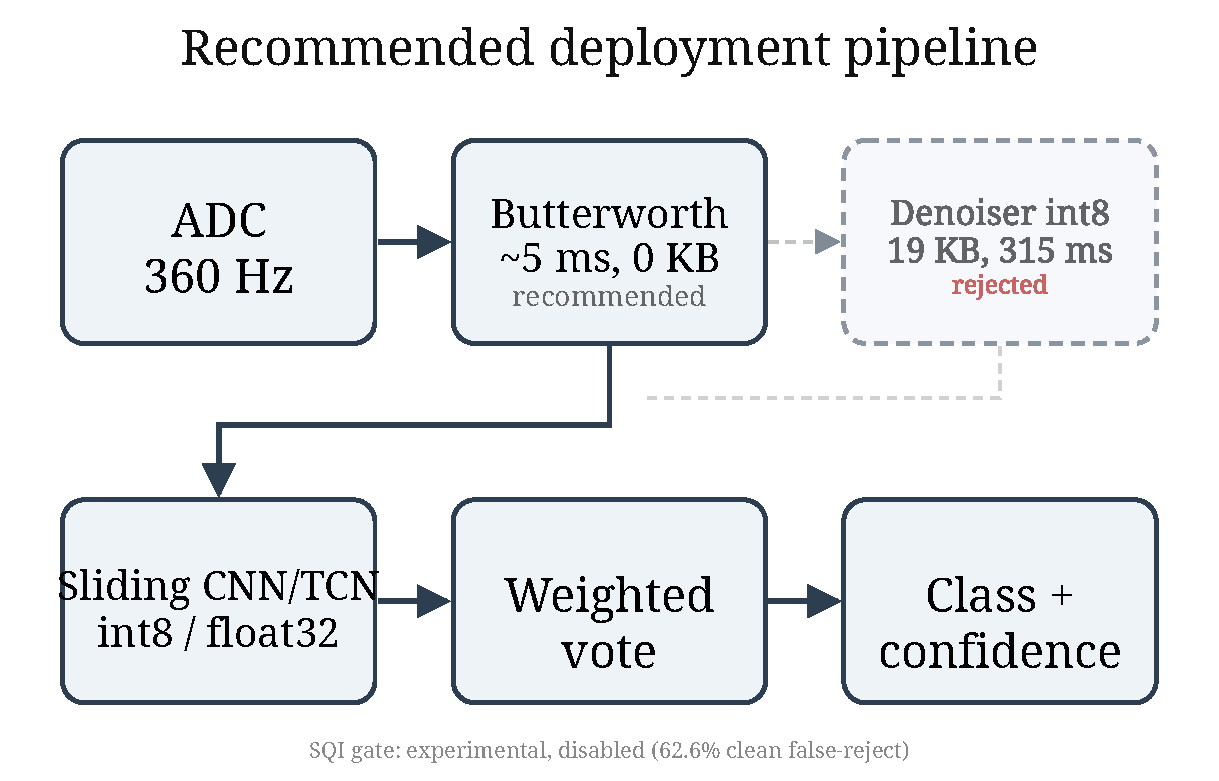
\includegraphics[width=0.88\columnwidth]{figures/fig_pipeline.pdf}
\caption{On-device inference pipeline on the ESP32-S3: ADC acquisition, signal-quality gate, quantized denoiser, sliding-window CNN classifier, confidence-weighted voting, and decision output.}
\label{fig:pipeline}
\end{figure}

\begin{equation}
S_c = \sum_{w} p_c^{(w)}, \qquad \hat{y} = \arg\max_c S_c, \qquad \mathrm{conf} = \frac{\max_c S_c}{\sum_c S_c}
\end{equation}

Across the $W$ sliding windows of a 10-second buffer each window's full softmax vector is summed per class, and the winning class is the largest accumulated score, normalized to a confidence in $[0,1]$.



\section{Experiments and Results}

Figure~\ref{fig:pipeline} shows the firmware-fixed pipeline. Exp.~1: grouped CV ($5\times2$, Table~\ref{tab:gcv}); Exp.~2: noise, SNR 0--40\,dB, 5 artifacts $\times$ 3 front-ends on the robust CNN (Table~\ref{tab:noise}, Fig.~\ref{fig:per_artifact}); Exp.~3: SVDB without retraining (Table~\ref{tab:svdb}); Exp.~4: paired FP32$\rightarrow$INT8 (Table~\ref{tab:compare}; Table~\ref{tab:deploy} reports fused-export sizes); Exp.~5: S3 memory/latency (Table~\ref{tab:deploy}, Fig.~\ref{fig:pareto}), calibration (Fig.~\ref{fig:calib}), SQI (Fig.~\ref{fig:sqi}). Exp.~2/4/calibration share one record-level split (918 windows: 493/24/401); Exp.~1 is the only $5\times2$ repeated evaluation.

\begin{table}[t]
\centering
\resizebox{\linewidth}{!}{
\begin{tabular}{lcccc}
\toprule
Model & Normal & APB & PVC & Macro \\
\midrule
CNN & 0.841 $\pm$ 0.145 & 0.283 $\pm$ 0.359 & 0.733 $\pm$ 0.369 & 0.619 $\pm$ 0.242 \\
TCN & 0.844 $\pm$ 0.147 & 0.257 $\pm$ 0.319 & 0.746 $\pm$ 0.368 & 0.615 $\pm$ 0.229 \\
LSTM & 0.792 $\pm$ 0.108 & 0.158 $\pm$ 0.221 & 0.796 $\pm$ 0.098 & 0.582 $\pm$ 0.096 \\
GRU & 0.728 $\pm$ 0.210 & 0.140 $\pm$ 0.203 & 0.709 $\pm$ 0.279 & 0.526 $\pm$ 0.170 \\
\bottomrule
\end{tabular}
}
\caption{Patient-independent $5$-fold $\times$ $2$-seed grouped CV (identical record-level folds for all architectures, $n=10$ folds per model). Mean $\pm$ SD; $95\%$ CI CNN $0.619\pm0.150$, TCN $0.615\pm0.142$, LSTM $0.582\pm0.060$, GRU $0.526\pm0.106$. APB support per fold varies (0--502 windows), explaining large SD.}
\label{tab:gcv}
\end{table}

\begin{table}[t]
\centering
\resizebox{\linewidth}{!}{
\begin{tabular}{l l c c c c}
\toprule
Model & Strategy & APB Prec & APB Rec & APB F1 & Macro \\
\midrule
CNN & baseline & 0.000 & 0.000 & 0.000 & 0.233 \\
CNN & weighted & 0.882 & 0.625 & \textbf{0.732} & 0.838 \\
CNN & focal & 0.425 & 0.708 & 0.531 & 0.818 \\
CNN & balanced & 0.929 & 0.542 & 0.684 & \textbf{0.876} \\
TCN & baseline & 0.875 & 0.583 & 0.700 & 0.753 \\
TCN & weighted & 0.750 & 0.625 & 0.682 & 0.876 \\
TCN & focal & 0.778 & 0.583 & 0.667 & 0.872 \\
TCN & balanced & 0.778 & 0.583 & 0.667 & 0.854 \\
LSTM & baseline & 0.143 & 0.042 & 0.065 & 0.299 \\
LSTM & weighted & 0.000 & 0.000 & 0.000 & 0.486 \\
LSTM & focal & 0.200 & 0.208 & 0.204 & 0.675 \\
LSTM & balanced & 0.019 & 0.042 & 0.026 & 0.305 \\
GRU & baseline & 0.000 & 0.000 & 0.000 & 0.237 \\
GRU & weighted & 0.200 & 0.375 & 0.261 & 0.642 \\
GRU & focal & 0.035 & 0.708 & 0.067 & 0.138 \\
GRU & balanced & 0.063 & 0.125 & 0.083 & 0.417 \\
\bottomrule
\end{tabular}
}
\caption{APB imbalance ablation (single record split, test $493/24/401$; $16$-way $=$ 4 architectures $\times$ 4 imbalance strategies). CNN weighted lifts APB $0\rightarrow0.732$; TCN already $0.70$ baseline. LSTM/GRU remain poor even with mitigation (best $0.26$), confirming architecture matters.}
\label{tab:apb}
\end{table}

\begin{table}[t]
\centering
\begin{tabular}{l l l l}
\toprule
SNR (dB) & Raw & Bandpass filter & Autoencoder \\
\midrule
0 & 0.233 & 0.455 & 0.475 \\
5 & 0.233 & 0.628 & 0.563 \\
10 & 0.286 & 0.726 & 0.586 \\
15 & 0.462 & 0.751 & 0.614 \\
20 & 0.683 & 0.723 & 0.629 \\
30 & 0.731 & 0.761 & 0.628 \\
40 & 0.736 & 0.751 & 0.629 \\
\bottomrule
\end{tabular}
\caption{Noise robustness on the robust CNN: macro F1 by front-end across SNR, averaged over the 5 artifact types.}
\label{tab:noise}
\end{table}

\begin{table}[t]
\centering
\resizebox{\linewidth}{!}{
\begin{tabular}{l c c c c c}
\toprule
Model & Float32 & Int8 & $\Delta$ & Disagree & Size (KB) \\
\midrule
CNN & 0.619 & 0.409 & $-0.210\pm0.164$ & 33.1\% & 77.9 \\
TCN & 0.615 & 0.378 & $-0.238\pm0.165$ & 39.7\% & 70.1 \\
LSTM & 0.582 & --- & --- & --- & 130.3 \\
GRU & 0.526 & --- & --- & --- & 107.5 \\
\bottomrule
\end{tabular}
}
\caption{Paired FP32$\rightarrow$INT8 on identical folds ($n=10$ per model, $5\times2$). INT8 degrades macro by $0.21$--$0.24$ (95\% CI $0.10$); LSTM/GRU not quantizable (\texttt{---}, TensorListStack, requires SELECT\_TF\_OPS). Disagree = fraction of all test windows whose argmax differs between FP32 and INT8. Single-split $0.588\rightarrow0.677$ (CNN) is split-specific, not paired. LSTM/GRU sizes are the SELECT\_TF\_OPS exports; Table~\ref{tab:deploy} benchmarks the smaller fused exports.}
\label{tab:compare}
\end{table}

Grouped CV (Table~\ref{tab:gcv}, $5\times2$ identical folds) shows CNN $0.619\pm0.242$ and TCN $0.615\pm0.229$ tied (CI overlapping), LSTM $0.582\pm0.096$, GRU $0.526\pm0.170$; APB support 0--502 per fold explains large SD. On the single held-out split (493/24/401, Table~\ref{tab:apb}), CNN baseline collapses on APB (F1 $0.000$); class weighting lifts it to $0.732$ (P $0.882$, R $0.625$) and balanced sampling gives $0.684$ at the best macro ($0.876$). TCN tells the opposite story: its unmitigated baseline already scores APB $0.700$---within rounding of CNN's best mitigated $0.732$---and every mitigation trades it away slightly for macro gain. LSTM/GRU's best APB is $0.261$ even with weighting, confirming architecture matters beyond loss balancing: TCN handles APB scarcity intrinsically, whereas CNN requires explicit rebalancing. Table~\ref{tab:apb} is a single-split mitigation ablation---an illustrative ceiling, not a generalization estimate: its test split contains only $24$ APB windows, and the $0.876$ macro reflects one favorable fold. Table~\ref{tab:gcv}'s $5\times2$ cross-validated average ($0.619$) is the honest number. SVDB has no APB, so we report N/V-macro $0.562$ (N $0.663$, PVC $0.462$, Table~\ref{tab:svdb}); 3-class $0.375$ is biased. Paired INT8 on identical folds (Table~\ref{tab:compare}) degrades macro by $0.210\pm0.164$ (CNN, 33\% disagree) and $0.238\pm0.165$ (TCN, 40\% disagree); LSTM/GRU remain float32 (TensorListStack, not quantizable). Calibration ($T=0.350$ fit on validation; held-out test, $n{=}918$) ECE $0.328\rightarrow0.051$, NLL $0.700\rightarrow0.407$, Brier $0.381\rightarrow0.210$ (Fig.~\ref{fig:calib}).

\begin{table}[t]
\centering
\begin{tabular}{l l l}
\toprule
Class & F1 & Windows \\
\midrule
Normal & 0.663 & 28{,}470 \\
APB & --- & 0 \\
PVC & 0.462 & 1{,}084 \\
N/V-macro & 0.562 & 29{,}554 \\
3-class (biased) & 0.375 & 29{,}554 \\
\bottomrule
\end{tabular}
\caption{External validation on SVDB (29{,}554 windows, 14 recordings). APB is absent (0 windows); its F1 enters the 3-class macro as 0 by definition, mechanically deflating it to $0.375$. We therefore report N/V-macro $0.562$ as the supported-class metric.}
\label{tab:svdb}
\end{table}

\begin{table}[t]
\centering
\resizebox{\linewidth}{!}{
\begin{tabular}{l c c c c c}
\toprule
Model & Macro & Size & Latency & RTF & $\Delta$INT8 \\
\midrule
CNN & 0.619 & 77.9 & 500 & 1.00 & $-0.210$ \\
TCN & 0.615 & 70.1 & 609 & 1.22 & $-0.238$ \\
LSTM & 0.582 & 126.5 & 1290 & 2.58 & --- \\
GRU & 0.526 & 103.7 & 1091 & 2.18 & --- \\
\bottomrule
\end{tabular}
}
\caption{Deployment master on ESP-NN-optimized kernels: grouped CV macro, flash size (KB; LSTM/GRU are the fused float32 exports of \S\ref{sec:methods-models}), measured per-window latency (ms, $n=19$ windows each, fixed-seed input, three runs, $<0.1\%$ spread; denoise $315$\,ms + classify remainder), RTF = per-window latency $\div$ 500\,ms hop (the streaming budget set by 50\% overlap; window-based values: 0.50/0.61/2.58/2.18), and paired INT8 $\Delta$. CNN and TCN meet the hop budget only once the learned denoiser is replaced by the ${\sim}5$\,ms Butterworth (\S IV-F). Arena $300$\,KB internal SRAM ($96$\,KB denoiser + $204$\,KB classifier), leaves $\approx49$\,KB heap by budget.}
\label{tab:deploy}
\end{table}

\subsection{On-Device Feasibility Verification}

The quantized CNN/TCN occupy $77.9$/$70.1$\,KB plus the $19$\,KB denoiser in flash; the float32 LSTM/GRU occupy $126.5$/$103.7$\,KB. The tensor arena is $300$\,KB internal SRAM, split $96$\,KB denoiser / $204$\,KB classifier to accommodate ESP-NN scratch; leaving $\approx49$\,KB heap by budget (Table~\ref{tab:deploy}, Fig.~\ref{fig:pareto}). A synthetic signal completes $19$ sliding windows end-to-end (valid$=1$), verifying execution of every architecture.

Measured per-window latency on \emph{ESP-NN-optimized kernels} (BENCHMARK\_MODE, $n=19$, $240$\,MHz, fixed-seed input, three runs each, variation $<0.1\%$): CNN $500$\,ms ($315$ denoise + $184$ classify), TCN $609$\,ms, LSTM $1290$\,ms, GRU $1091$\,ms. Against the streaming budget set by the 0.5-s hop, the denoiser-in-loop pipeline is marginal: CNN sits exactly at RTF $1.00$ and TCN exceeds it ($1.22$), and the batch firmware would occupy $95\%$ duty cycle per 10-s buffer. Replacing the learned denoiser with the ${\sim}5$\,ms Butterworth---already favored on cost--benefit grounds---resolves this decisively: classify-only latency falls to $189$/$298$\,ms (hop-based RTF $0.38$/$0.60$, $36\%$ duty cycle), so \emph{CNN and TCN meet real-time precisely because the denoiser must go}; float32 LSTM/GRU fail under either framing ($\geq1.55$). Outputs were verified bit-exact against PC reference kernels, whereas TFL-Micro's portable reference kernels had run the conv stacks $7.6\times$/$5.9\times$ slower---inverting the ranking. Kernel optimization, not architecture, was the bottleneck: ESP-NN accelerates int8 convolution ${\approx}17\times$ while float32 sequence kernels gain only ${\sim}20\%$. Notably, esp-nn v1.0.0's S3 assembly kernels produced silently incorrect conv outputs on our shapes; our fixed-input hardware A/B harness localized the fault, and upstream master fixes resolve it. The denoiser stage drops $595\rightarrow315$\,ms; the ${\sim}5$\,ms Butterworth remains favorable. DAC$\rightarrow$ADC replay (hardware-domain $\Delta$F1) is impossible on S3 (no DAC; \texttt{SOC\_DAC\_SUPPORTED}=0) --- see Limitations.

% ponytail: fig_confusion/gcv/noise/compare moved to supplementary to meet 6-page IEEE limit; pareto/calibration/per-artifact/sqi are the primary deployment figures
% \begin{figure}[t]\centering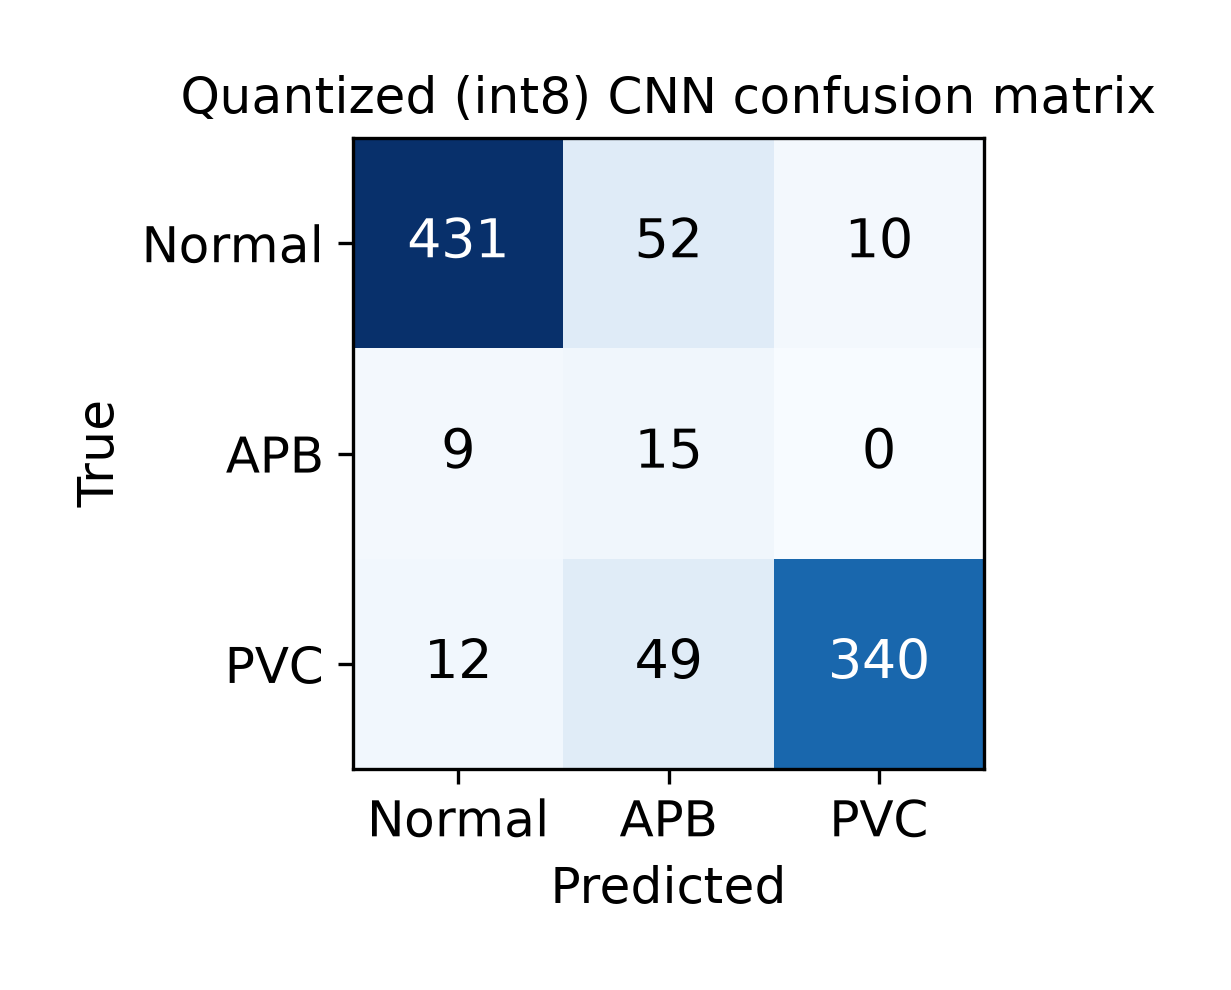
\includegraphics[width=0.98\columnwidth]{figures/fig_confusion.png}\caption{...}\label{fig:confusion}\end{figure}
% \begin{figure}[t]\centering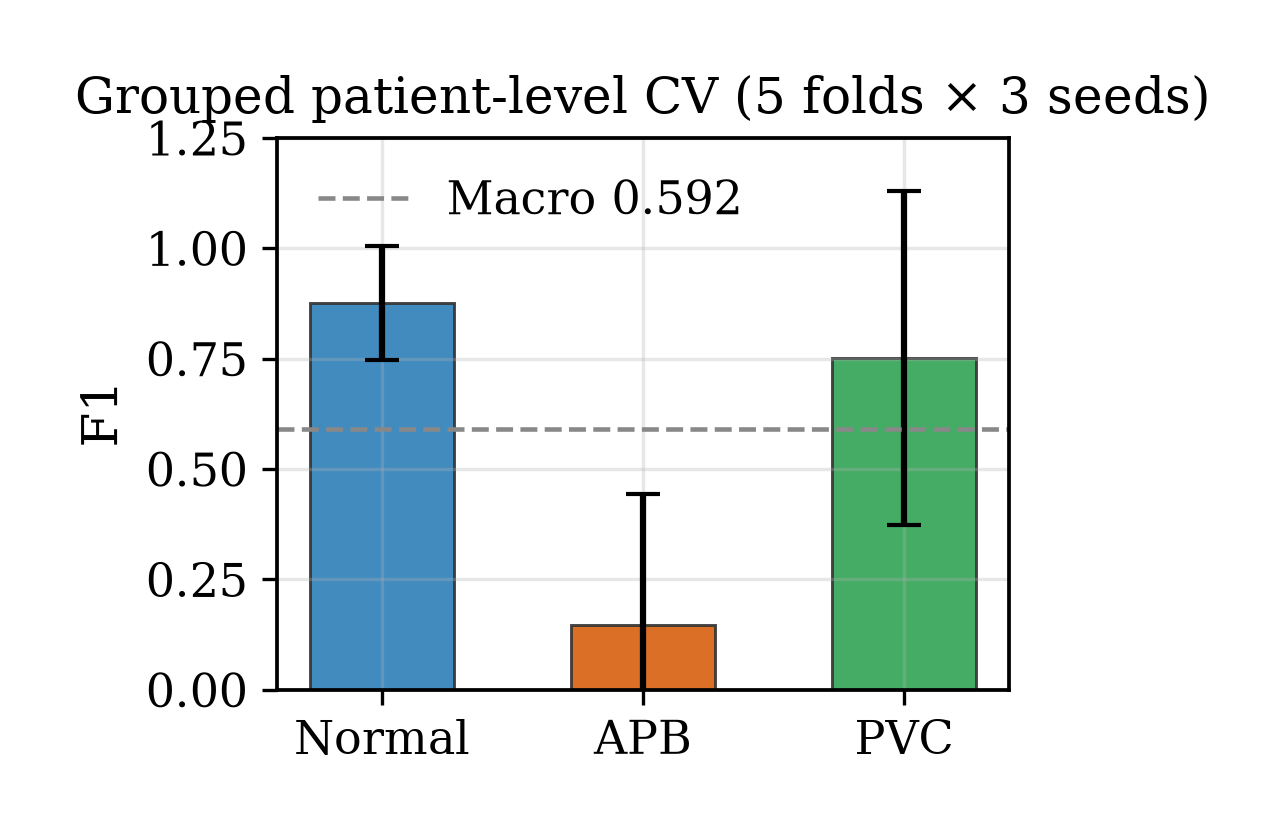
\includegraphics[width=0.98\columnwidth]{figures/fig_gcv.png}\caption{...}\label{fig:gcv}\end{figure}
% \begin{figure}[t]\centering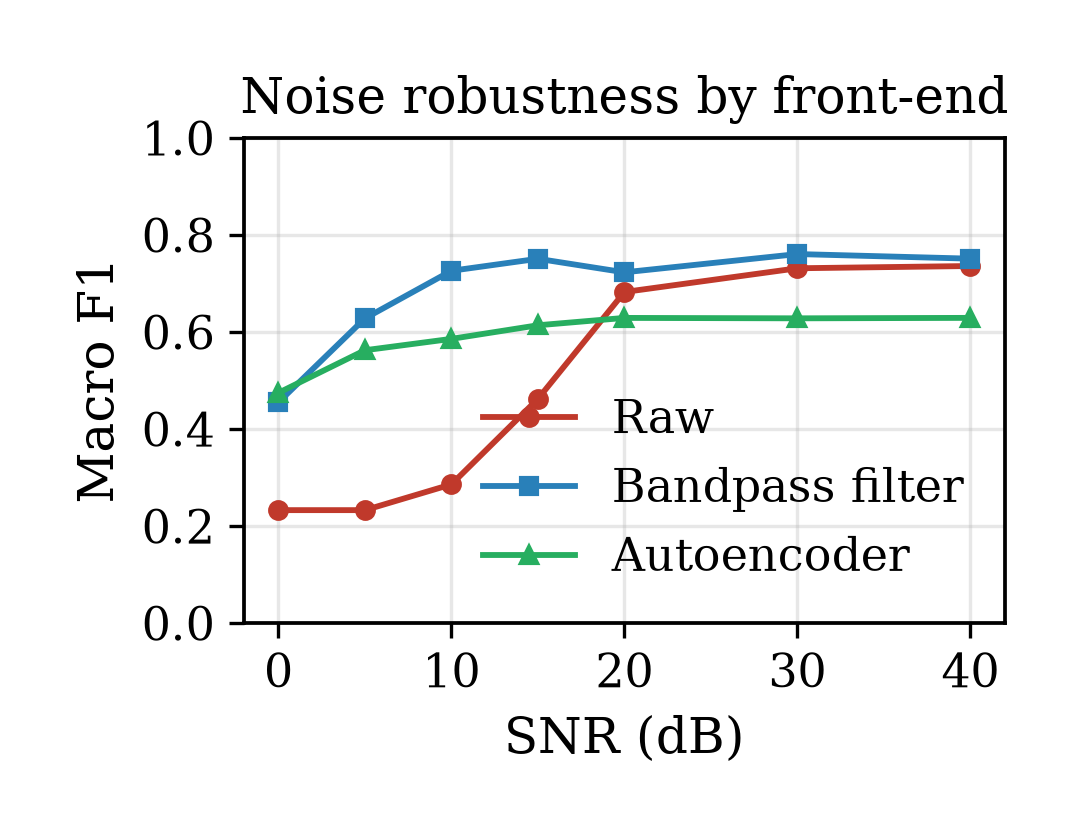
\includegraphics[width=0.98\columnwidth]{figures/fig_noise.png}\caption{...}\label{fig:noise}\end{figure}
% \begin{figure}[t]\centering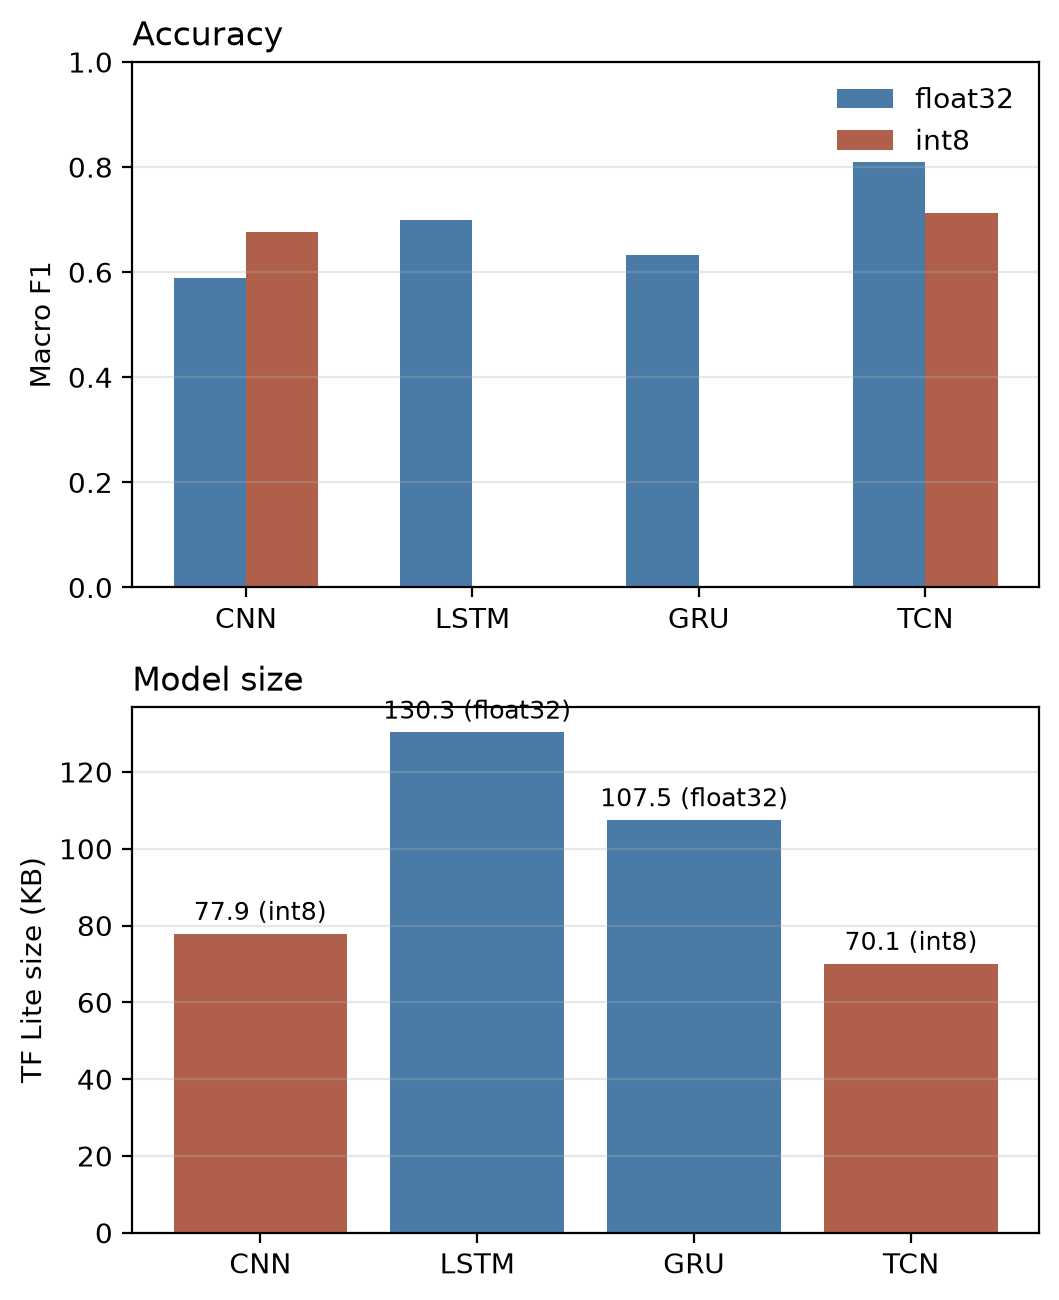
\includegraphics[width=\columnwidth]{figures/fig_compare.png}\caption{...}\label{fig:compare}\end{figure}

\begin{figure}[t]
\centering
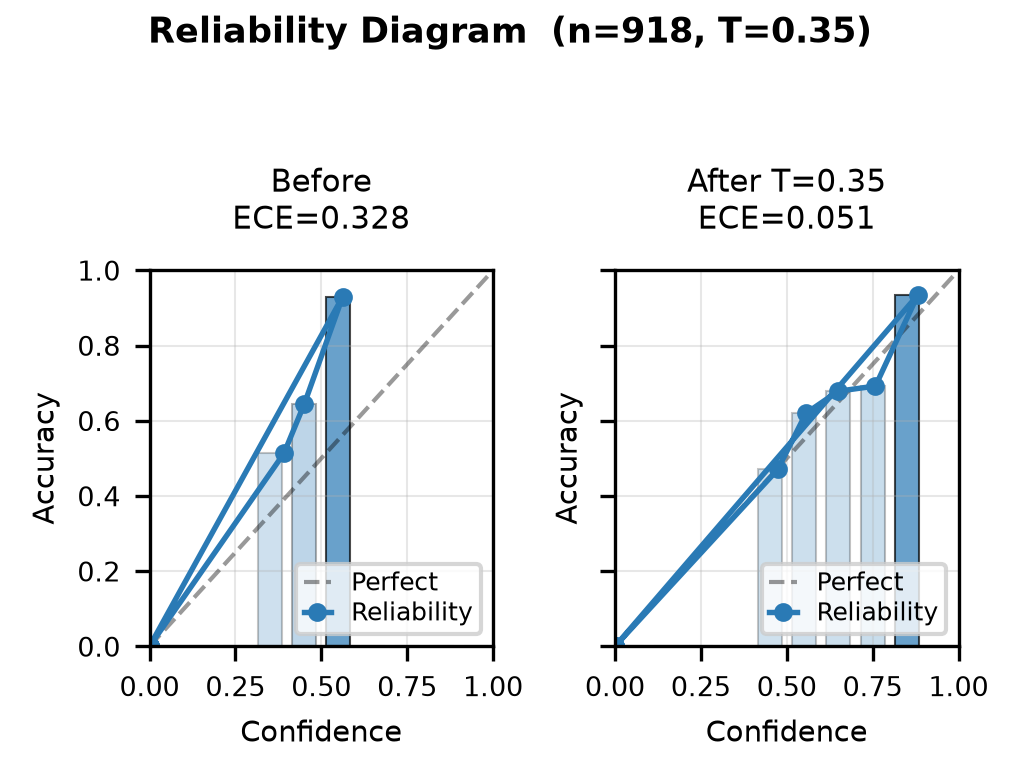
\includegraphics[width=0.90\columnwidth]{figures/fig_calib.png}
\caption{Calibration reliability diagram (robust CNN; $T=0.350$ fit on validation, evaluated on held-out test, $n{=}918$). ECE $0.328\rightarrow0.051$, NLL $0.700\rightarrow0.407$, Brier $0.381\rightarrow0.210$ — 10 bins, bar opacity = count.}
\label{fig:calib}
\end{figure}

\begin{figure}[t]
\centering
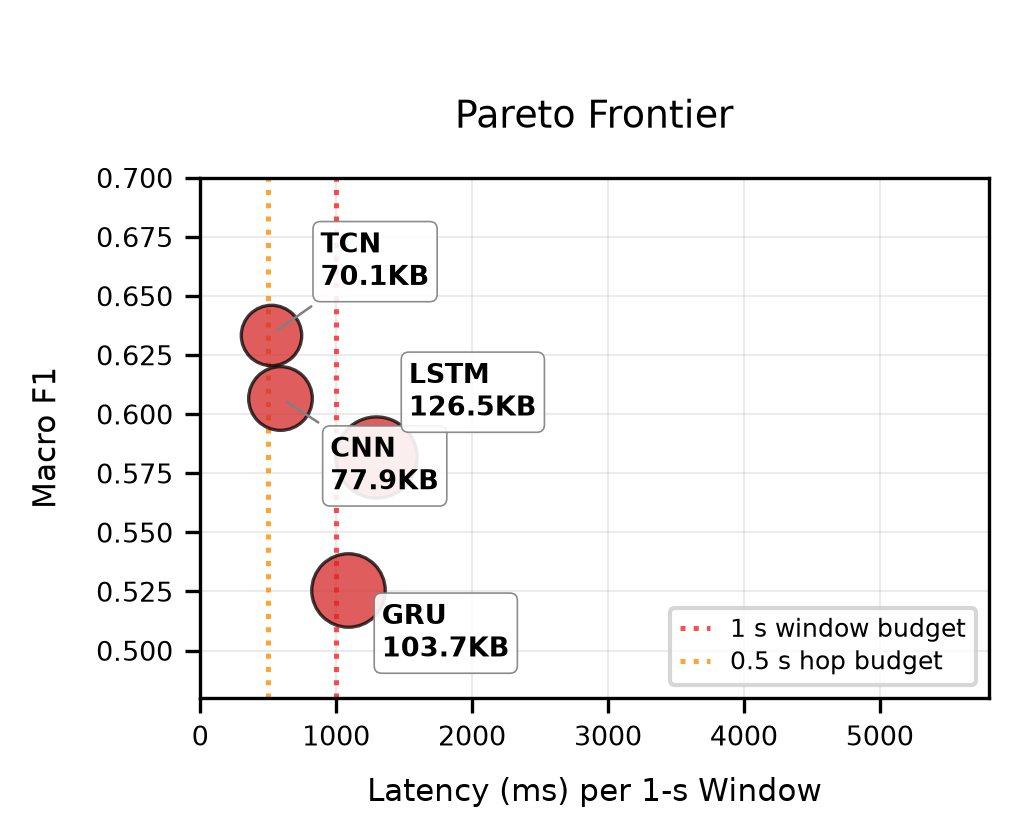
\includegraphics[width=0.90\columnwidth]{figures/fig_pareto.png}
\caption{Pareto: grouped CV macro vs. measured ESP-NN per-window latency. Dashed budgets: 1-s window and 0.5-s overlap hop. CNN/TCN meet the hop budget only without the learned denoiser (\S IV-F); float32 LSTM/GRU remain above both.}
\label{fig:pareto}
\end{figure}

\begin{figure}[t]
\centering
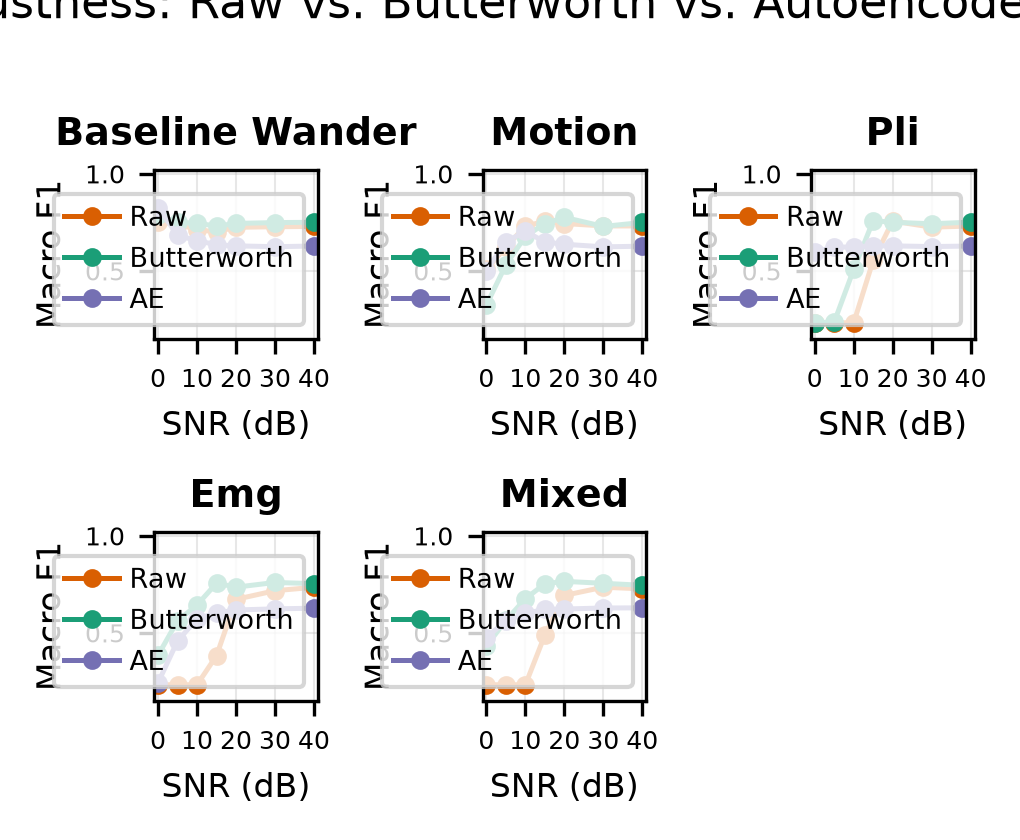
\includegraphics[width=0.80\columnwidth]{figures/fig_per_artifact.png}
\caption{Per-artifact robustness ($5$ types $\times$ $7$ SNR, single-column 3 rows: 2+2+1). Butterworth wins 3/5, raw wins motion, AE only wins PLI low-SNR — denoiser not justified.}
\label{fig:per_artifact}
\end{figure}

\begin{figure}[t]
\centering
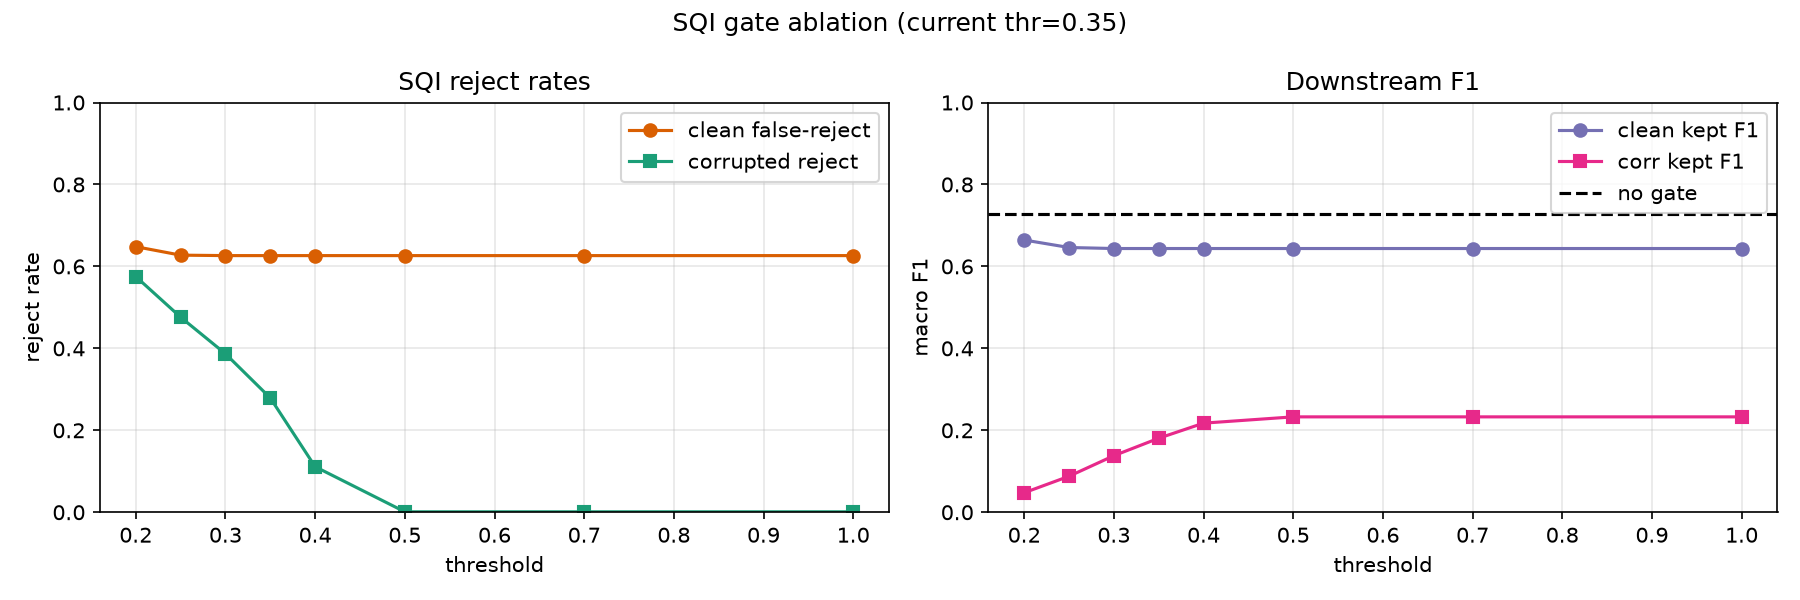
\includegraphics[width=0.90\columnwidth]{figures/fig_sqi.png}
\caption{SQI gate: clean false-reject $62.6\%$ at $0.35$, corrupted reject $27.9\%$, downstream macro $0.727\rightarrow0.643$ — gate as tuned not deployable.}
\label{fig:sqi}
\end{figure}

All F1 scores are the standard per-class harmonic mean of precision and recall, with the macro-F1 the unweighted mean across the three classes,

\begin{equation}
F1_c = \frac{2\,\mathrm{TP}_c}{2\,\mathrm{TP}_c + \mathrm{FP}_c + \mathrm{FN}_c}, \qquad \mathrm{Macro\text{-}F1} = \frac{1}{C}\sum_{c=1}^{C} F1_c
\end{equation}


\section{Discussion and Limitations}

Single-lead limits scope (no ST localization/axis). APB is beat-level, not AF (rhythm-level, scoped out). On-device we report a functional smoke test ($19$ windows) and measured latency (Table~\ref{tab:deploy}); hardware-domain $\Delta$F1 via DAC$\rightarrow$ADC replay is impossible on S3 (no DAC), and real AD8232 acquisition and battery life remain future hardware/ethics work.

Grouped CV ($5\times2$ identical folds, Table~\ref{tab:gcv}) ties CNN $0.619\pm0.242$ and TCN $0.615\pm0.229$ (CI overlapping), LSTM $0.582\pm0.096$, GRU $0.526\pm0.170$; PVC SD $0.37$ reflects fold composition, not penalty. Noise: Butterworth wins $3/5$ artifacts, raw wins motion, the AE only low-SNR PLI (Fig.~\ref{fig:per_artifact}); its $19$\,KB + $315$\,ms buys $<0.1$ macro. The SQI gate rejects $62.6\%$ clean vs. $27.9\%$ corrupted at $0.35$ (Fig.~\ref{fig:sqi}) --- not deployable without retuning. Quantization (Table~\ref{tab:compare}) costs $0.21$--$0.24$ macro with $33$/$40\%$ disagreement, arguing for calibrated-confidence abstention.

Deployment (Table~\ref{tab:deploy}) on ESP-NN-optimized kernels: against the 0.5-s hop budget, CNN/TCN are marginal with the denoiser in-loop (RTF $1.00$/$1.22$) and comfortably real-time without it ($0.38$/$0.60$); float32 LSTM/GRU remain above budget and unquantizable. Memory is not the limiter (PSRAM unused). The esp-nn v1.0.0 numerical fault caught during this work (silent conv corruption on S3 shapes, fixed upstream) argues for probability-level on-device validation whenever kernel libraries are swapped.

Older MIT-BIH literature reports $\ge0.90$ accuracy, but with patient overlap. Our patient-level GroupKFold ($5\times2$) keeps recordings disjoint; APB scarcity drives low macro and are the honest new-patient numbers ($0.53$--$0.62$ across architectures) vs. patient-specific $\ge0.90$ \cite{kiranyaz2016,acharya2017,hannun2019}.

Reproducibility: PhysioNet pull \cite{goldberger2000,mitdb,greenwaldsvdb}, frozen $5\times2$ folds, 96 retained checkpoints, seeds documented; TensorFlow 2.21 / Keras 3 / scikit-learn \cite{pedregosa2011}; firmware header conversion and BENCHMARK\_MODE share the tree; all tables/figs regenerate end-to-end. On-device figures use an in-tree ESP-NN build; LSTM/GRU timings use fused float32 exports with unchanged weights.

\section{Conclusion}

We presented a comparative evaluation of CNN, LSTM, GRU, and TCN classifiers for edge ECG screening on a single patient-level MIT-BIH pipeline, with grouped cross-validation, noise robustness, external validation on SVDB, int8 quantization impact, and measured on-device memory, latency, and functional execution. On ESP32-S3 with ESP-NN-optimized kernels, CNN and TCN meet the streaming real-time budget (hop-based RTF $0.38$/$0.60$) once the denoiser is replaced by a Butterworth filter---upgraded by this analysis from cost preference to hard requirement---at a modest footprint, with outputs matching PC reference. Float32 LSTM/GRU exceed budget under either framing and are unquantizable: kernel-aware architecture choice settles the accuracy--latency trade-off in favor of small conv stacks.



\section*{Use of a Large Language Model (LLM) in the Manuscript}
The authors hereby declare that the use of ChatGPT or any LLM in the preparation of this research paper is either not applicable, or if utilized, has been duly acknowledged within the paper (preferably in the 'ACKNOWLEDGEMENT' Section), where it is explicitly stated that such models were employed solely for non-intellectual purposes. The authors confirm that the output generated by ChatGPT or any LLM has been carefully reviewed and approved by them. The responsibility for the content and accuracy of the information rests solely with the authors.
\FloatBarrier
\bibliographystyle{IEEEtran}
\bibliography{references}

\end{document}